\documentclass{ximera}
\title{Introduction to Polynomial Functions}

\outcome{Determine the end behavior of a polynomial from its leading term.}
\outcome{Find zeros of a polynomial and state their multiplicities.}
\outcome{Use the Intermediate Value Theorem to locate zeros.}
\outcome{Write a polynomial function from given zeros and a point.}

\begin{document}
\begin{abstract}
\end{abstract}
\maketitle

\textbf{Learning Objectives:}
\begin{itemize}
  \item Determine the end behavior of a polynomial from its leading term.
  \item Find zeros of a polynomial and state their multiplicities.
  \item Use the Intermediate Value Theorem to locate zeros.
  \item Write a polynomial function from given zeros and a point.
\end{itemize}
\medskip

\noindent\textbf{Intermediate Value Theorem (IVT) for Polynomials:} If $f$ is a polynomial and $f(a)$ and $f(b)$ have opposite signs for $a<b$, then $f$ has at least one zero in $[a,b]$.

\bigskip
\section*{Quick Check}

\begin{problem}
Given polynomial $p(x) = -3(x-4)^2(2x+1)(1-x)^3$, which statement is true?
\begin{hint}
Find the leading term by multiplying the leading term of each factor.
\end{hint}
\begin{multipleChoice}
  \choice{The range of $p(x)$ is $(-\infty,\infty)$.}
  \choice{As $x\to\pm\infty$, $p(x)\to-\infty$.}
  \choice[correct]{As $x\to+\infty$, $p(x)\to+\infty$.}
  \choice{The graph crosses the $x$-axis at $x=4$.}
  \choice{$p(x)$ has a zero at $x=-1$.}
\end{multipleChoice}
\end{problem}

\begin{problem}
Which polynomial function has a zero for which the graph \emph{touches but does not cross} the $x$-axis?
\begin{hint}
A graph touches (but does not cross) at a zero with even multiplicity.
\end{hint}
\begin{multipleChoice}
  \choice{$m(x) = x^3 - 9x$}
  \choice{$m(x) = -2(x-3)(4x+1)^3$}
  \choice[correct]{$m(x) = x^4 - x^2$}
  \choice{$m(x) = 3x^5 + 12x$}
\end{multipleChoice}
\end{problem}

\begin{problem}
Determine the leading term of $f(x) = -2(x+5)(1-x)^3(3x+2)^2$.
\begin{hint}
Multiply the leading terms of each factor: $(-2)(x)(-x)^3(3x)^2$.
\end{hint}
\begin{multipleChoice}
  \choice{$-2x$}
  \choice{$6x^3$}
  \choice[correct]{$18x^6$}
  \choice{$-9x^6$}
\end{multipleChoice}
\end{problem}

\begin{problem}
The graph below shows $f(x) = (x+2)^2(x-1)$.

\begin{center}
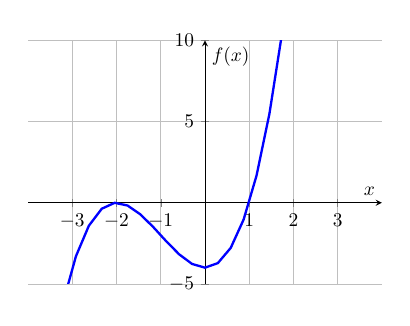
\begin{tikzpicture}[scale=0.7]
\begin{axis}[
  axis lines=middle,
  xmin=-4, xmax=4,
  ymin=-5, ymax=10,
  xtick={-3,-2,-1,0,1,2,3},
  ytick={-5,0,5,10},
  grid=both,
  width=8cm, height=6cm,
  xlabel={$x$}, ylabel={$f(x)$}
]
\addplot[very thick, blue, domain=-3.5:3.5] {(x+2)^2*(x-1)};
\end{axis}
\end{tikzpicture}
\end{center}

Which statement about $f(x)$ is true?
\begin{hint}
Check the multiplicity of each zero and whether the graph crosses or touches at that zero.
\end{hint}
\begin{multipleChoice}
  \choice{$x=2$ is a zero of even multiplicity; the graph crosses there.}
  \choice[correct]{$x=-2$ is a zero of even multiplicity; the graph touches there.}
  \choice{$x=-2$ is a zero of odd multiplicity; the graph touches there.}
  \choice{$x=1$ is a zero of even multiplicity; the graph touches there.}
\end{multipleChoice}
\end{problem}

\begin{problem}
How many distinct $x$-intercepts does $f(x) = x^5 - 4x^3$ have?
\begin{hint}
Factor completely: $x^5-4x^3 = x^3(x^2-4)$.
\end{hint}
\begin{multipleChoice}
  \choice{1}
  \choice{2}
  \choice[correct]{3}
  \choice{4}
\end{multipleChoice}
\end{problem}


\bigskip
\section*{Extended Practice}

\begin{problem}
Let $g(x) = 2x^3 - 13x^2 + 18x + 5$.
\begin{enumerate}
  \item[(a)] Evaluate $g(2)$ and $g(3)$.
  \medskip
  \item[(b)] Use the IVT to determine whether $g(x)$ has a zero in $[2,3]$. Justify your answer.
\end{enumerate}

\begin{solution}
\begin{enumerate}
  \item[(a)] $g(2) = 16-52+36+5 = 5$; $\quad g(3) = 54-117+54+5 = -4$.

  \item[(b)] $g(2)=5>0$ and $g(3)=-4<0$ have opposite signs, and $g$ is a polynomial (hence continuous). By the IVT, $g$ has at least one zero in $[2,3]$.
\end{enumerate}
\end{solution}
\end{problem}


\begin{problem}
Determine the end behavior of each function.
\begin{enumerate}
  \item[(a)] $\ds g(x) = -\dfrac{1}{2}x^6 + 8x^4 - x^3 + 9$
  \medskip
  \item[(b)] $n(x) = 2(x+4)(3x-1)^3(x+5)$
  \medskip
  \item[(c)] $f(x) = -5x^4(2-x)^3(2x+5)$
\end{enumerate}

\begin{solution}
\begin{enumerate}
  \item[(a)] Leading term: $-\frac{1}{2}x^6$ (degree 6, even; leading coeff $<0$).\\
  As $x\to\pm\infty$: $g(x)\to-\infty$.

  \item[(b)] Leading term: $2(x)(3x)^3(x) = 54x^5$ (degree 5, odd; leading coeff $>0$).\\
  As $x\to-\infty$: $n(x)\to-\infty$; as $x\to+\infty$: $n(x)\to+\infty$.

  \item[(c)] Leading term: $-5x^4(-x)^3(2x) = -5x^4(-x^3)(2x) = 10x^8$ (degree 8, even; leading coeff $>0$).\\
  As $x\to\pm\infty$: $f(x)\to+\infty$.
\end{enumerate}
\end{solution}
\end{problem}


\begin{problem}
Find the zeros of each function and state their multiplicities.
\begin{enumerate}
  \item[(a)] $g(x) = x^3 + 5x^2 - x - 5$
  \medskip
  \item[(b)] $k(x) = 4x^4 - 65x^2 + 16$
  \medskip
  \item[(c)] $f(x) = x^6 + 4x^5 + 4x^4$
  \medskip
  \item[(d)] $h(x) = -2x^4(x+1)^3(x-2)^2$
  \medskip
  \item[(e)] $z(x) = 4x(5x-1)(3x+8)(x-\sqrt{5})(x+\sqrt{5})$
\end{enumerate}

\begin{solution}
\begin{enumerate}
  \item[(a)] Factor by grouping: $x^2(x+5)-1(x+5) = (x+5)(x^2-1) = (x+5)(x-1)(x+1)$.\\
  Zeros: $x=-5,\; x=1,\; x=-1$, all with multiplicity 1.

  \item[(b)] $4x^4-65x^2+16 = (x^2-16)(4x^2-1) = (x-4)(x+4)(2x-1)(2x+1)$.\\
  Zeros: $x=4,\; x=-4,\; x=\frac{1}{2},\; x=-\frac{1}{2}$, all with multiplicity 1.

  \item[(c)] $x^4(x^2+4x+4) = x^4(x+2)^2$.\\
  Zeros: $x=0$ (multiplicity 4), $x=-2$ (multiplicity 2).

  \item[(d)] Zeros: $x=0$ (multiplicity 4), $x=-1$ (multiplicity 3), $x=2$ (multiplicity 2).

  \item[(e)] Zeros: $x=0,\; x=\frac{1}{5},\; x=-\frac{8}{3},\; x=\sqrt{5},\; x=-\sqrt{5}$, all with multiplicity 1.
\end{enumerate}
\end{solution}
\end{problem}


\begin{problem}
Write a polynomial function $y = f(x)$ whose graph could match the given graph (aside from vertical scaling).
\begin{enumerate}
  \item[(a)]

\begin{center}
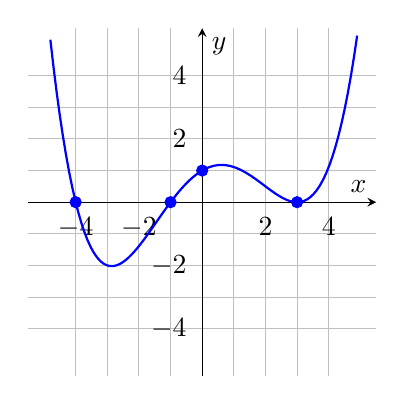
\begin{tikzpicture}
\begin{axis}[
  axis lines=center, width=6cm, height=6cm,
  xlabel={$x$}, ylabel={$y$},
  xmin=-5.5, xmax=5.5, xtick={-4,-2,0,2,4},
  ymin=-5.5, ymax=5.5, ytick={-4,-2,0,2,4},
  grid=both, minor tick num=1, tick style={draw=none},
]
\addplot[thick, blue, domain=-4.8:4.9, samples=100] {(x+4)*(x+1)*(x-3)^2/36};
\addplot[only marks, mark=*, blue] coordinates {(-4,0) (-1,0) (0,1) (3,0)};
\end{axis}
\end{tikzpicture}
\end{center}

  \medskip
  \item[(b)]

\begin{center}
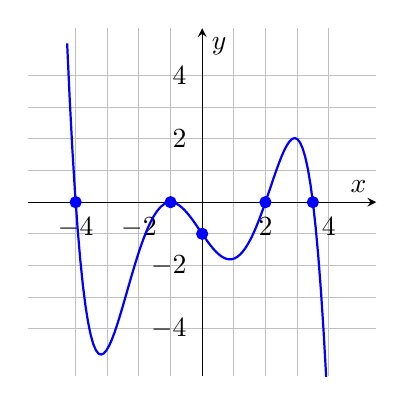
\begin{tikzpicture}
\begin{axis}[
  axis lines=center, width=6cm, height=6cm,
  xlabel={$x$}, ylabel={$y$},
  xmin=-5.5, xmax=5.5, xtick={-4,-2,0,2,4},
  ymin=-5.5, ymax=5.5, ytick={-4,-2,0,2,4},
  grid=both, minor tick num=1, tick style={draw=none},
]
\addplot[thick, blue, domain=-4.27:3.92, samples=100] {-(x+4)*(x+1)^2*(x-2)*(x-3.5)/28};
\addplot[only marks, mark=*, blue] coordinates {(-4,0) (-1,0) (0,-1) (2,0) (3.5,0)};
\end{axis}
\end{tikzpicture}
\end{center}
\end{enumerate}

\begin{solution}
\begin{enumerate}
  \item[(a)] Zeros: $x=-4$ (crosses, mult 1), $x=-1$ (crosses, mult 1), $x=3$ (touches, mult 2). So $f(x) = a(x+4)(x+1)(x-3)^2$. Use the $y$-intercept $(0,1)$:
  $$1 = a(4)(1)(9) \implies a = \frac{1}{36}$$
  So $f(x) = \dfrac{1}{36}(x+4)(x+1)(x-3)^2$.

  \item[(b)] Zeros: $x=-4$ (crosses, mult 1), $x=-1$ (touches, mult 2), $x=2$ (crosses, mult 1), $x=3.5$ (crosses, mult 1). So $f(x) = a(x+4)(x+1)^2(x-2)(x-3.5)$. Use the $y$-intercept $(0,-1)$:
  $$-1 = a(4)(1)(-2)(-3.5) = 28a \implies a = -\frac{1}{28}$$
  So $f(x) = -\dfrac{1}{28}(x+4)(x+1)^2(x-2)(x-3.5)$.
\end{enumerate}
\end{solution}
\end{problem}


\begin{problem}
For each polynomial, identify the zeros, their multiplicities, the end behavior, and the $y$-intercept, then sketch the graph.
\begin{enumerate}
  \item[(a)] $m(x) = 0.1(x-3)^2(x+1)^3$
  \medskip
  \item[(b)] $g(x) = x^4 - x^3 - 6x^2$
\end{enumerate}

\begin{solution}
\begin{enumerate}
  \item[(a)] $m(x) = 0.1(x-3)^2(x+1)^3$
  \begin{itemize}
    \item Zeros: $x=3$ (mult 2, touches); $x=-1$ (mult 3, crosses).
    \item Leading term: $0.1x^5$ (degree 5, odd; positive leading coeff). As $x\to-\infty$: $m\to-\infty$; as $x\to+\infty$: $m\to+\infty$.
    \item $y$-intercept: $m(0) = 0.1(9)(1) = 0.9$.
  \end{itemize}

\begin{center}
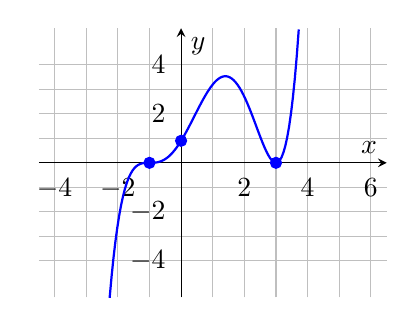
\begin{tikzpicture}
\begin{axis}[
  axis lines=center, width=6cm, height=5cm,
  xlabel={$x$}, ylabel={$y$},
  xmin=-4.5, xmax=6.5, xtick={-4,-2,0,2,4,6},
  ymin=-5.5, ymax=5.5, ytick={-4,-2,0,2,4},
  grid=both, minor tick num=1, tick style={draw=none},
]
\addplot[thick, blue, domain=-2.26:3.72, samples=100] {0.1*(x-3)^2*(x+1)^3};
\addplot[only marks, mark=*, blue] coordinates {(-1,0) (0,0.9) (3,0)};
\end{axis}
\end{tikzpicture}
\end{center}

  \item[(b)] $g(x) = x^4-x^3-6x^2 = x^2(x^2-x-6) = x^2(x-3)(x+2)$
  \begin{itemize}
    \item Zeros: $x=0$ (mult 2, touches); $x=3$ (mult 1, crosses); $x=-2$ (mult 1, crosses).
    \item Leading term: $x^4$ (degree 4, even; positive). As $x\to\pm\infty$: $g\to+\infty$.
    \item $y$-intercept: $(0,0)$.
  \end{itemize}

\begin{center}
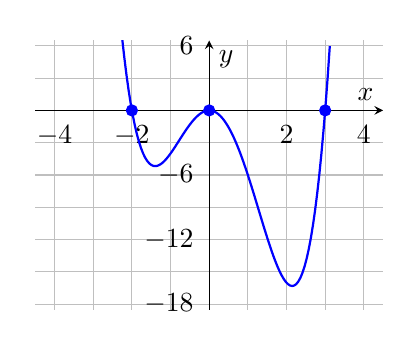
\begin{tikzpicture}
\begin{axis}[
  axis lines=center, width=6cm, height=5cm,
  xlabel={$x$}, ylabel={$y$},
  xmin=-4.5, xmax=4.5, xtick={-4,-2,0,2,4},
  ymin=-18.5, ymax=6.5, ytick={-18,-12,-6,0,6},
  grid=both, minor tick num=1, tick style={draw=none},
]
\addplot[thick, blue, domain=-2.25:3.12, samples=100] {x^4-x^3-6*x^2};
\addplot[only marks, mark=*, blue] coordinates {(-2,0) (0,0) (3,0)};
\end{axis}
\end{tikzpicture}
\end{center}
\end{enumerate}
\end{solution}
\end{problem}

\end{document}
